\section{Introduction}
\label{slab:sec:intro}

Chapter~1 posed the question that drives this chapter: can whole-query
rewriting work with no rules at all? Chapter~2 explained why the
question is worth asking. Rule-based rewriters, however carefully
curated, are bounded by their rule sets; a query whose optimization
opportunity falls outside every rule's pattern is a query they cannot
improve. Chapter~2 also laid out the ingredients an answer would need:
if rewriting is framed as search, then finding a better query means
enumerating candidate formulations and admitting only those that can
be shown equivalent to the original, using the spectrum of testing,
bounded verification, and full verification.

Framing the problem this way is easy; making the search succeed is
not. The space of queries equivalent to a given input is unbounded,
and almost all of the syntactically valid candidates in it are not
equivalent at all. An enumerative synthesizer that walks this space in
order of size, the standard discipline in program synthesis, spends
its entire budget rejecting nonsense before it encounters the first
interesting candidate. Worse, rejecting a candidate is itself
expensive: equivalence must be disproved, and although a
cheap-to-costly checking pipeline softens the blow, no pipeline is
cheap enough to absorb an undirected search. And even that is not the
full requirement. An equivalent query is only useful if it is also
faster, so the search must surface not one equivalent formulation but
enough of them that a faster one is likely among them. What the search
needs is direction: a signal, computable from the input query alone,
that says which regions of the space are worth entering.

This chapter's answer is the \emph{query dataflow}, and it is the
central contribution of this dissertation to the \slabcity project. A
dataflow is a semantic abstraction of a query: a description of how
information moves from base tables through the query's operations to
its output, stripped of the syntactic packaging in which the movement
is expressed. Two observations make dataflows the right search signal.
First, dataflows can be extracted from a query mechanically, by
analysis of the query alone, before any search begins. Second, and
more importantly, semantically related queries are connected through
the dataflows they share. If a query computes an aggregate and filters
on it, any equivalent formulation almost certainly performs the same
essential computation somewhere, however differently it is spelled.
Equivalence lives at the level of what a query computes, and dataflows
capture what a query computes. A candidate that shares the input
query's dataflows is a plausible relative; a candidate that exhibits
none of them is almost certainly a stranger, and the search can treat
it accordingly.

\slabcity is the system that turns this signal into a rewriter, and it
was built jointly with Rui Dong. The division of work, stated here
because this dissertation presents the project from one side of it, is
as follows. The dataflow abstraction is the contribution of this
dissertation: the definition of dataflows for SQL queries, the
procedure for extracting them, and the observation that equivalent
queries are connected through shared dataflows. The synthesis
machinery that consumes the abstraction is Rui Dong's contribution:
the scoring function that turns shared dataflows into a numeric
priority over candidates, and the enumerative synthesis algorithm that
uses that priority to stratify and prune the search. This chapter
therefore develops the dataflow abstraction in full and presents the
synthesis machinery in summary, with the
publication~\cite{dong2023slabcity} as the complete reference. The
remaining components were developed in close collaboration, and the
evaluation was carried out jointly.

\begin{figure}
\centering
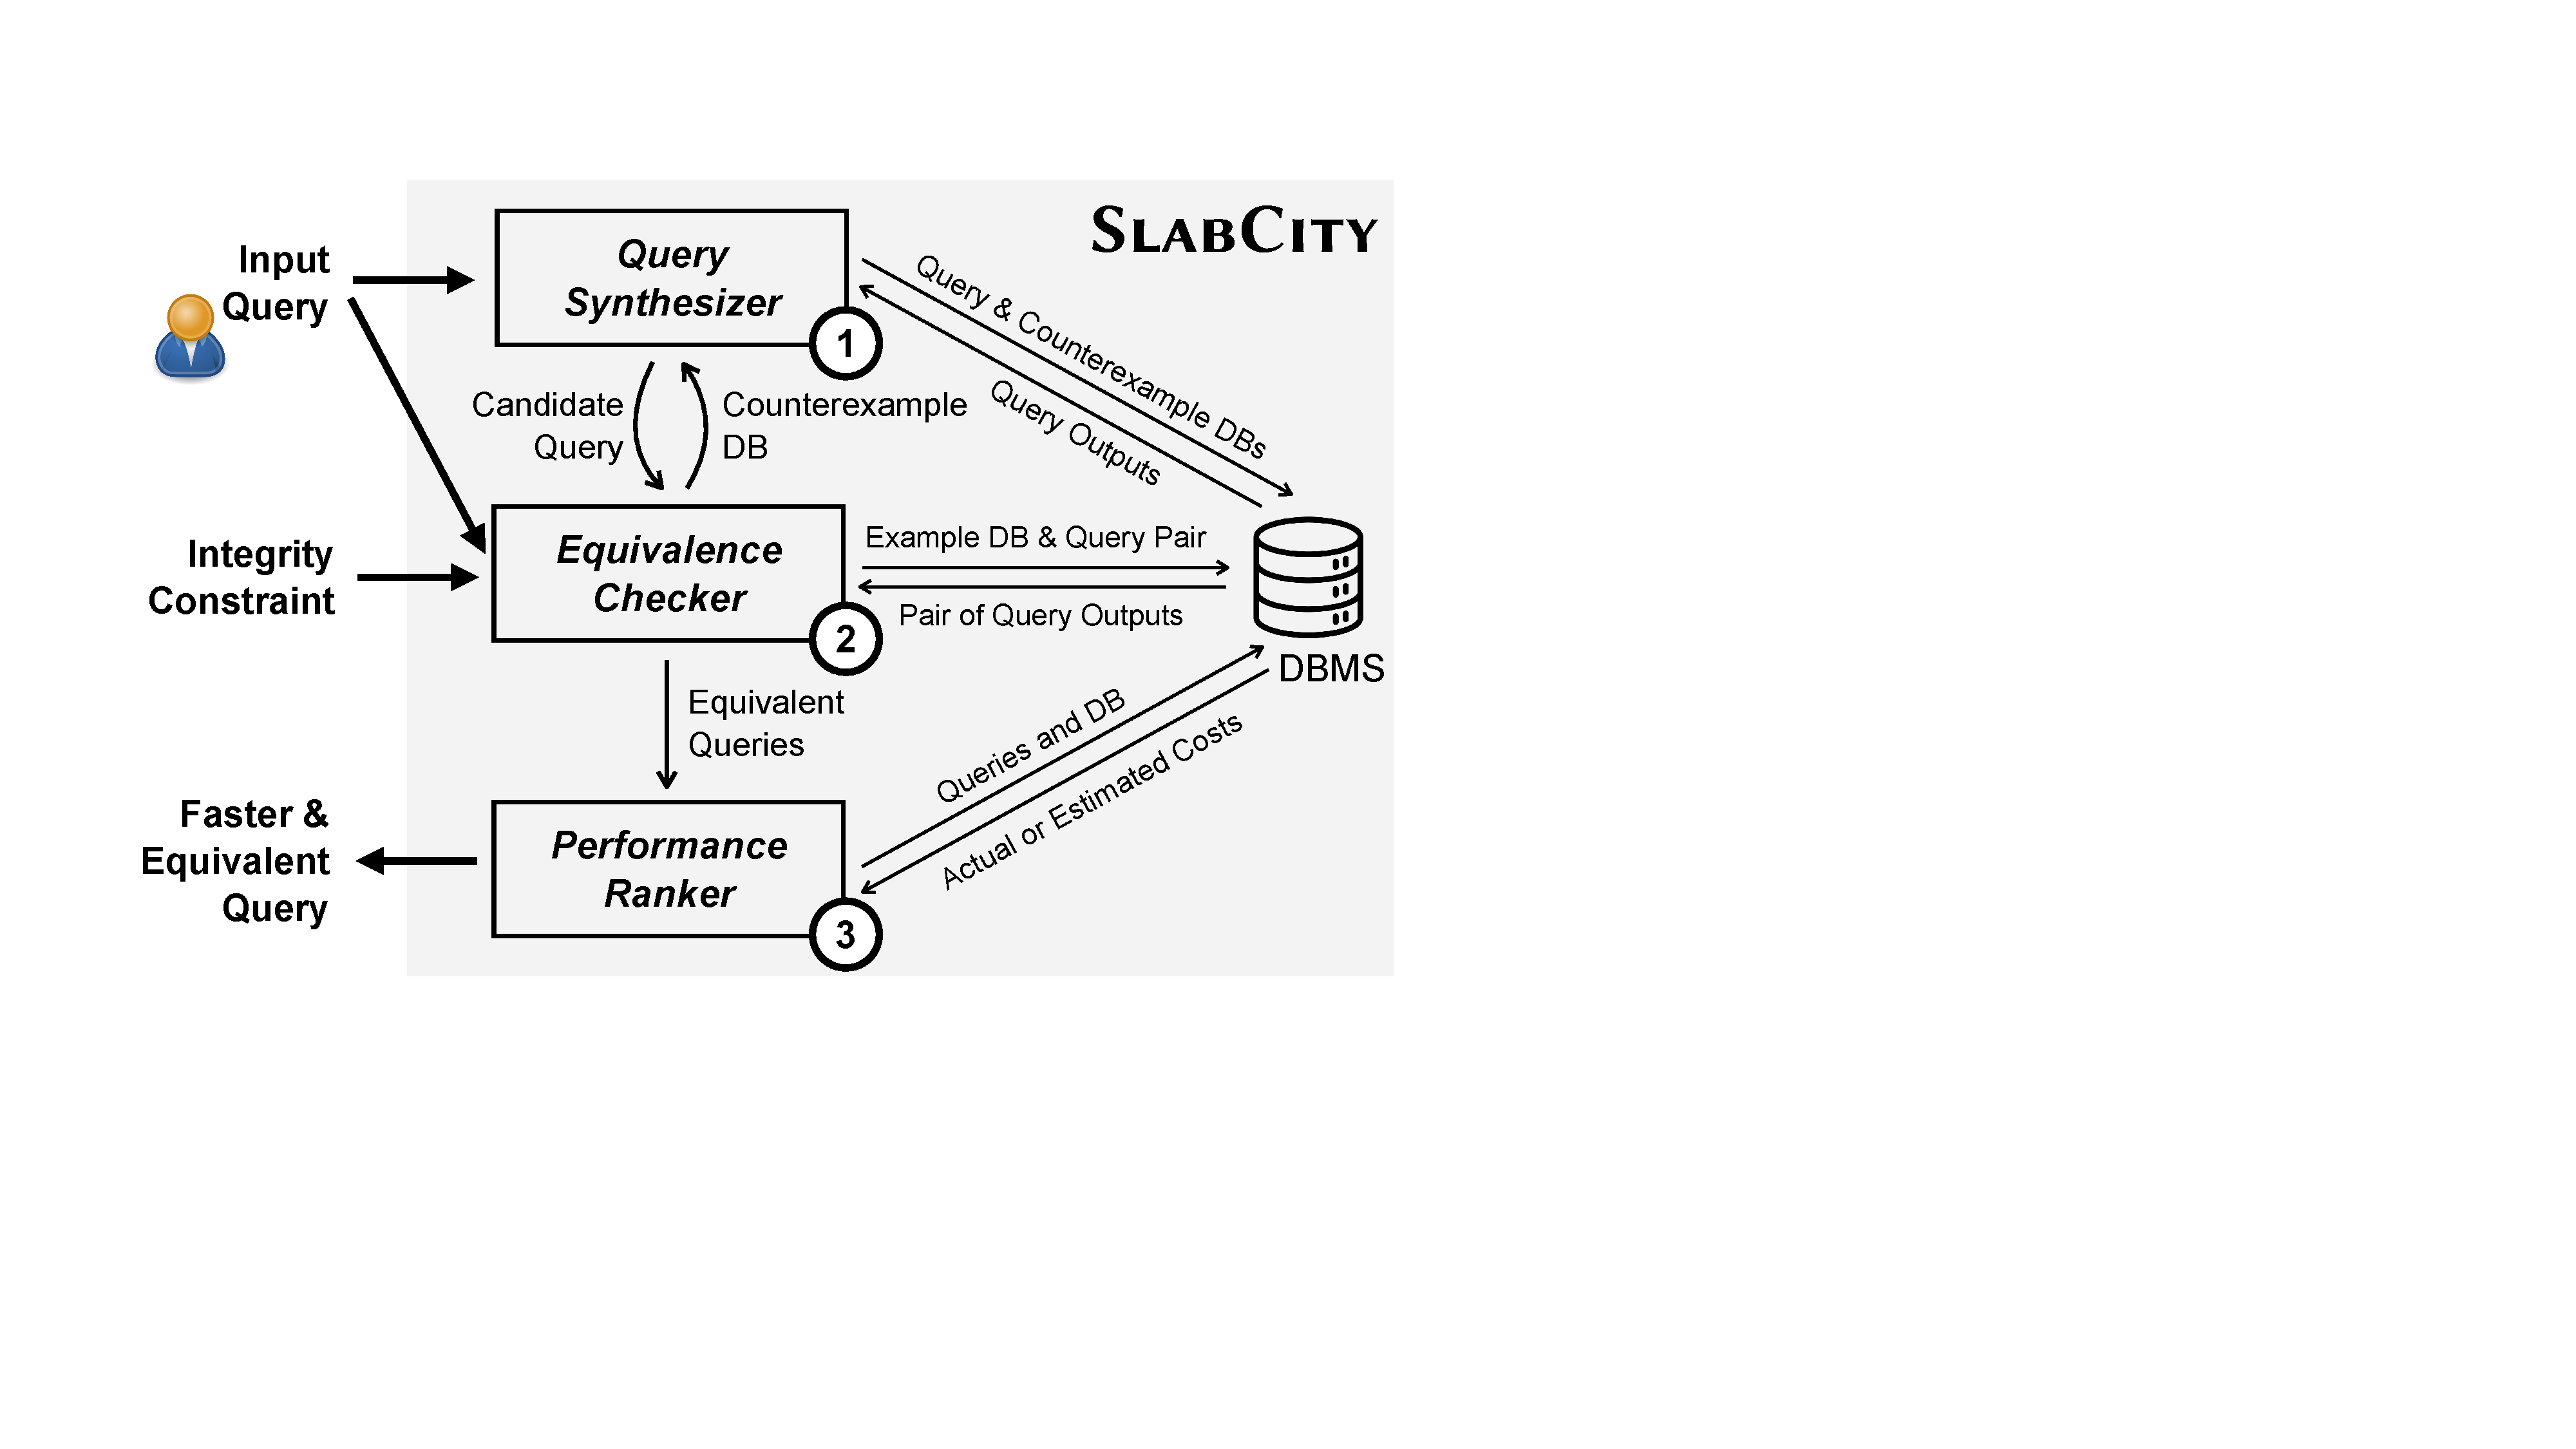
\includegraphics[width=0.8\linewidth]{chapters/slabcity/figs/workflow-clean.pdf}
\vspace{-5pt}
\caption{Schematic workflow of \slabcity.}
\vspace{-10pt}
\label{slab:fig:workflow}
\end{figure}

At the system level, \slabcity takes a query and the integrity
constraints of its schema and returns a semantically equivalent query
expected to run faster. \Cref{slab:fig:workflow} shows the
architecture, which instantiates the counterexample-guided inductive
synthesis (CEGIS) loop introduced in Chapter~2. A dataflow-guided
synthesizer proposes candidates that agree with the input query on all
counterexample databases collected so far. Each candidate then faces
the layered equivalence checker: a fast tester that hunts for a
distinguishing database, a bounded verifier that proves agreement on
all small inputs, and a full verifier that, when it succeeds within
its budget, establishes equivalence outright. A candidate refuted by
the tester or by the bounded verifier yields a new counterexample
database that sharpens the synthesizer's next proposals; a refutation
by the full verifier arrives as a verdict rather than a witness, and
simply discards the candidate. A candidate that survives is labeled
with the strongest guarantee it earned: fully verified, verified on
all bounded inputs, or, when the verifiers cannot reach a conclusion
within their budgets, tested. Surviving candidates are ranked by
measured or estimated latency, and the fastest is returned with its
label; a fully verified rewrite can be deployed as is, while the
weaker labels route the rewrite for human inspection.

\slabcity is aimed at workloads where a few seconds of one-time search
effort is negligible against the query's lifetime cost. That covers
queries written once and executed indefinitely, dashboards and the
query templates embedded in database-backed applications, and it
covers long-running analytical queries, where even a single execution
dwarfs a five-second rewriting budget. In both settings the rewriter
runs as a deployment-time step, after the query is written and before
it enters service. The supported language is an expressive subset of
SQL, including nested subqueries and arbitrary join structure; the
formal definition appears in \cref{slab:sec:problem}.

In summary, this chapter makes the following contributions:
\begin{itemize}[leftmargin=*]
\item
It introduces query dataflows: a semantic abstraction of SQL queries,
an algorithm for extracting the dataflows a query manifests, and the
observation that equivalent queries share dataflows, which converts an
undirected search space into a navigable one (a contribution of this
dissertation).
\item
It presents \slabcity, the first synthesis-based rewriter capable of
whole-query optimization with no rewrite rules, combining
dataflow-guided synthesis (due to Rui Dong, summarized here) with
layered equivalence checking (joint work).
\item
It contributes a benchmark of more than 1{,}000 real-life queries
curated from LeetCode, supporting research on query rewriting beyond
this chapter (joint work).
\item
It evaluates \slabcity against state-of-the-art rule-based and learned
rewriters across four workloads, showing that it optimizes 7 to 68\%
more queries and produces rewrites up to four orders of magnitude
faster (joint work).
\end{itemize}

The rest of the chapter proceeds as follows.
\Cref{slab:sec:motivating-example} illustrates, through queries drawn
from real workloads, the rewrites that rule-based systems miss and
this chapter's approach finds. \Cref{slab:sec:problem} defines the
query language and the rewriting problem precisely.
\Cref{slab:sec:dataflow} develops the dataflow abstraction, the
technical core of the chapter. \Cref{slab:sec:synthesis} summarizes
how the synthesis algorithm consumes dataflows to drive the search,
and \cref{slab:sec:eval} presents the evaluation. Related work,
including the two prior systems that apply synthesis to query
rewriting under rule-based or locality
restrictions~\cite{zhou2021sia,wang2022optimizing}, is discussed in
\cref{chap:related}.
